\newpage
\section*{Responses}

\begin{itemize}

\item Idea is akin to holdout samples (in computer science, but also social sciences \citep{liu_successes_2019}) 
\item "common task framework": research design from machine learning called the common task method \citep{donoho_50_2017,liberman_obituary_2010}. The common task method involves three main elements: a common target for predictive modeling, a common error metric, and a common data set with both training data available to participants and held-out data used for evaluation. \citep{liu_successes_2019}

\end{itemize}

\textbf{General responses}

\begin{response}
    Thank you to the editor and the reviewers for their valuable input, which I very much appreciated, and which I believe has lead to substantial improvement of the text. I have revised the structure of the text, and linked it with various other efforts highlighted by the reviewers. 

    \begin{itemize}
        \item I have added a new introduction that lays out what the article intends to convey, and what tools it will describe. This should help make it clearer from the start, and should have been included; my apologies for only adding it now.
        \item I then follow with a section that describes and situates the various concepts, both those that might be new to some in the readership (``containers'') and those that might be known, but possibly ambiguously defined and used in a broader context (first among them: ``synthetic data''). This was a request by multiple reviewers, suggesting that it is still a necessary structure to provide. I will note that I had previously talked with others in the open (social) science field, who very much implied that even the late definition of containers was ``very pedantic'' because apparently everybody (should) know about that by now... highlighting the wide diversity in information dispersal even within the narrow "field" of social science. I hope that the current definitions strike a good balance.
        \item I have also replaced Figure 1 with a better figure, referenced it in the text, and added Figure 5, which shows the equivalent process flow for the Docker-based approach. For reference, here are the old Figure 1 and the new Figure 1 side-by-side (Figure~\ref{fig:comparision}.
    \end{itemize}
\end{response}

\begin{figure}
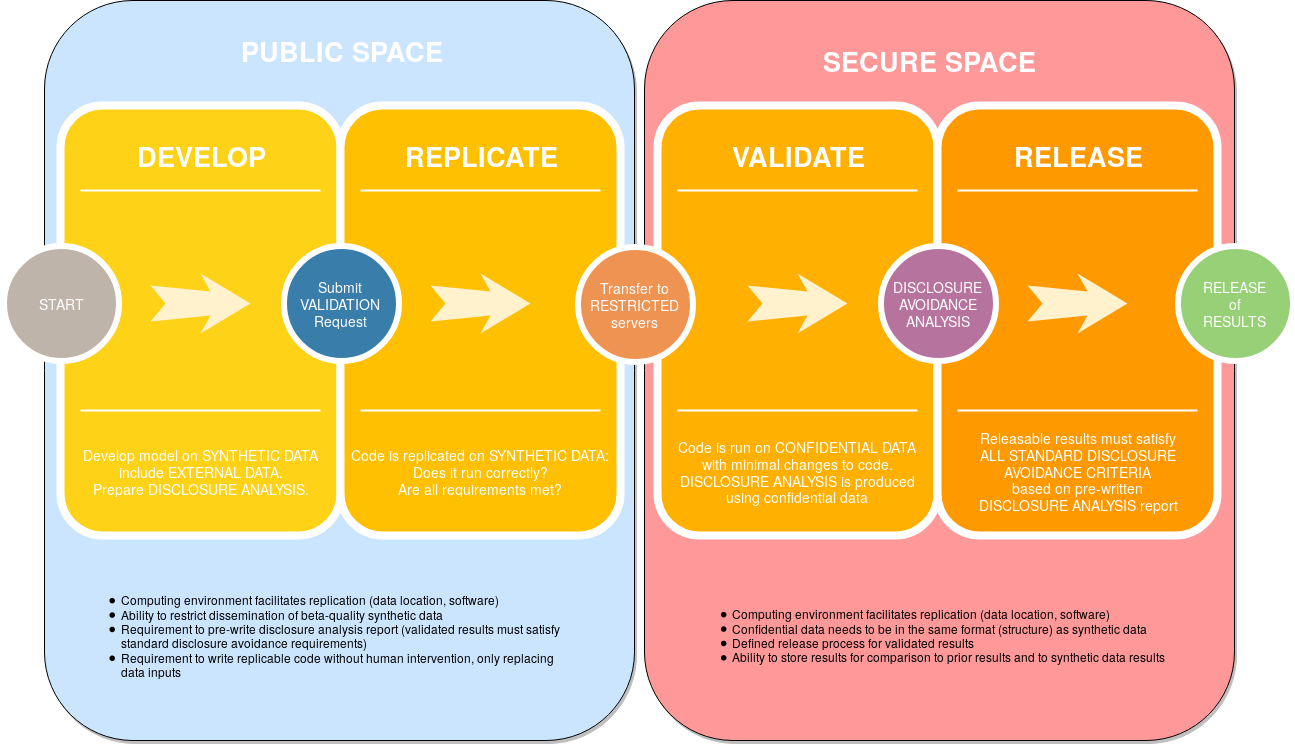
\includegraphics[width=0.45\textwidth]{figs/SyntheticDataCycle.png}
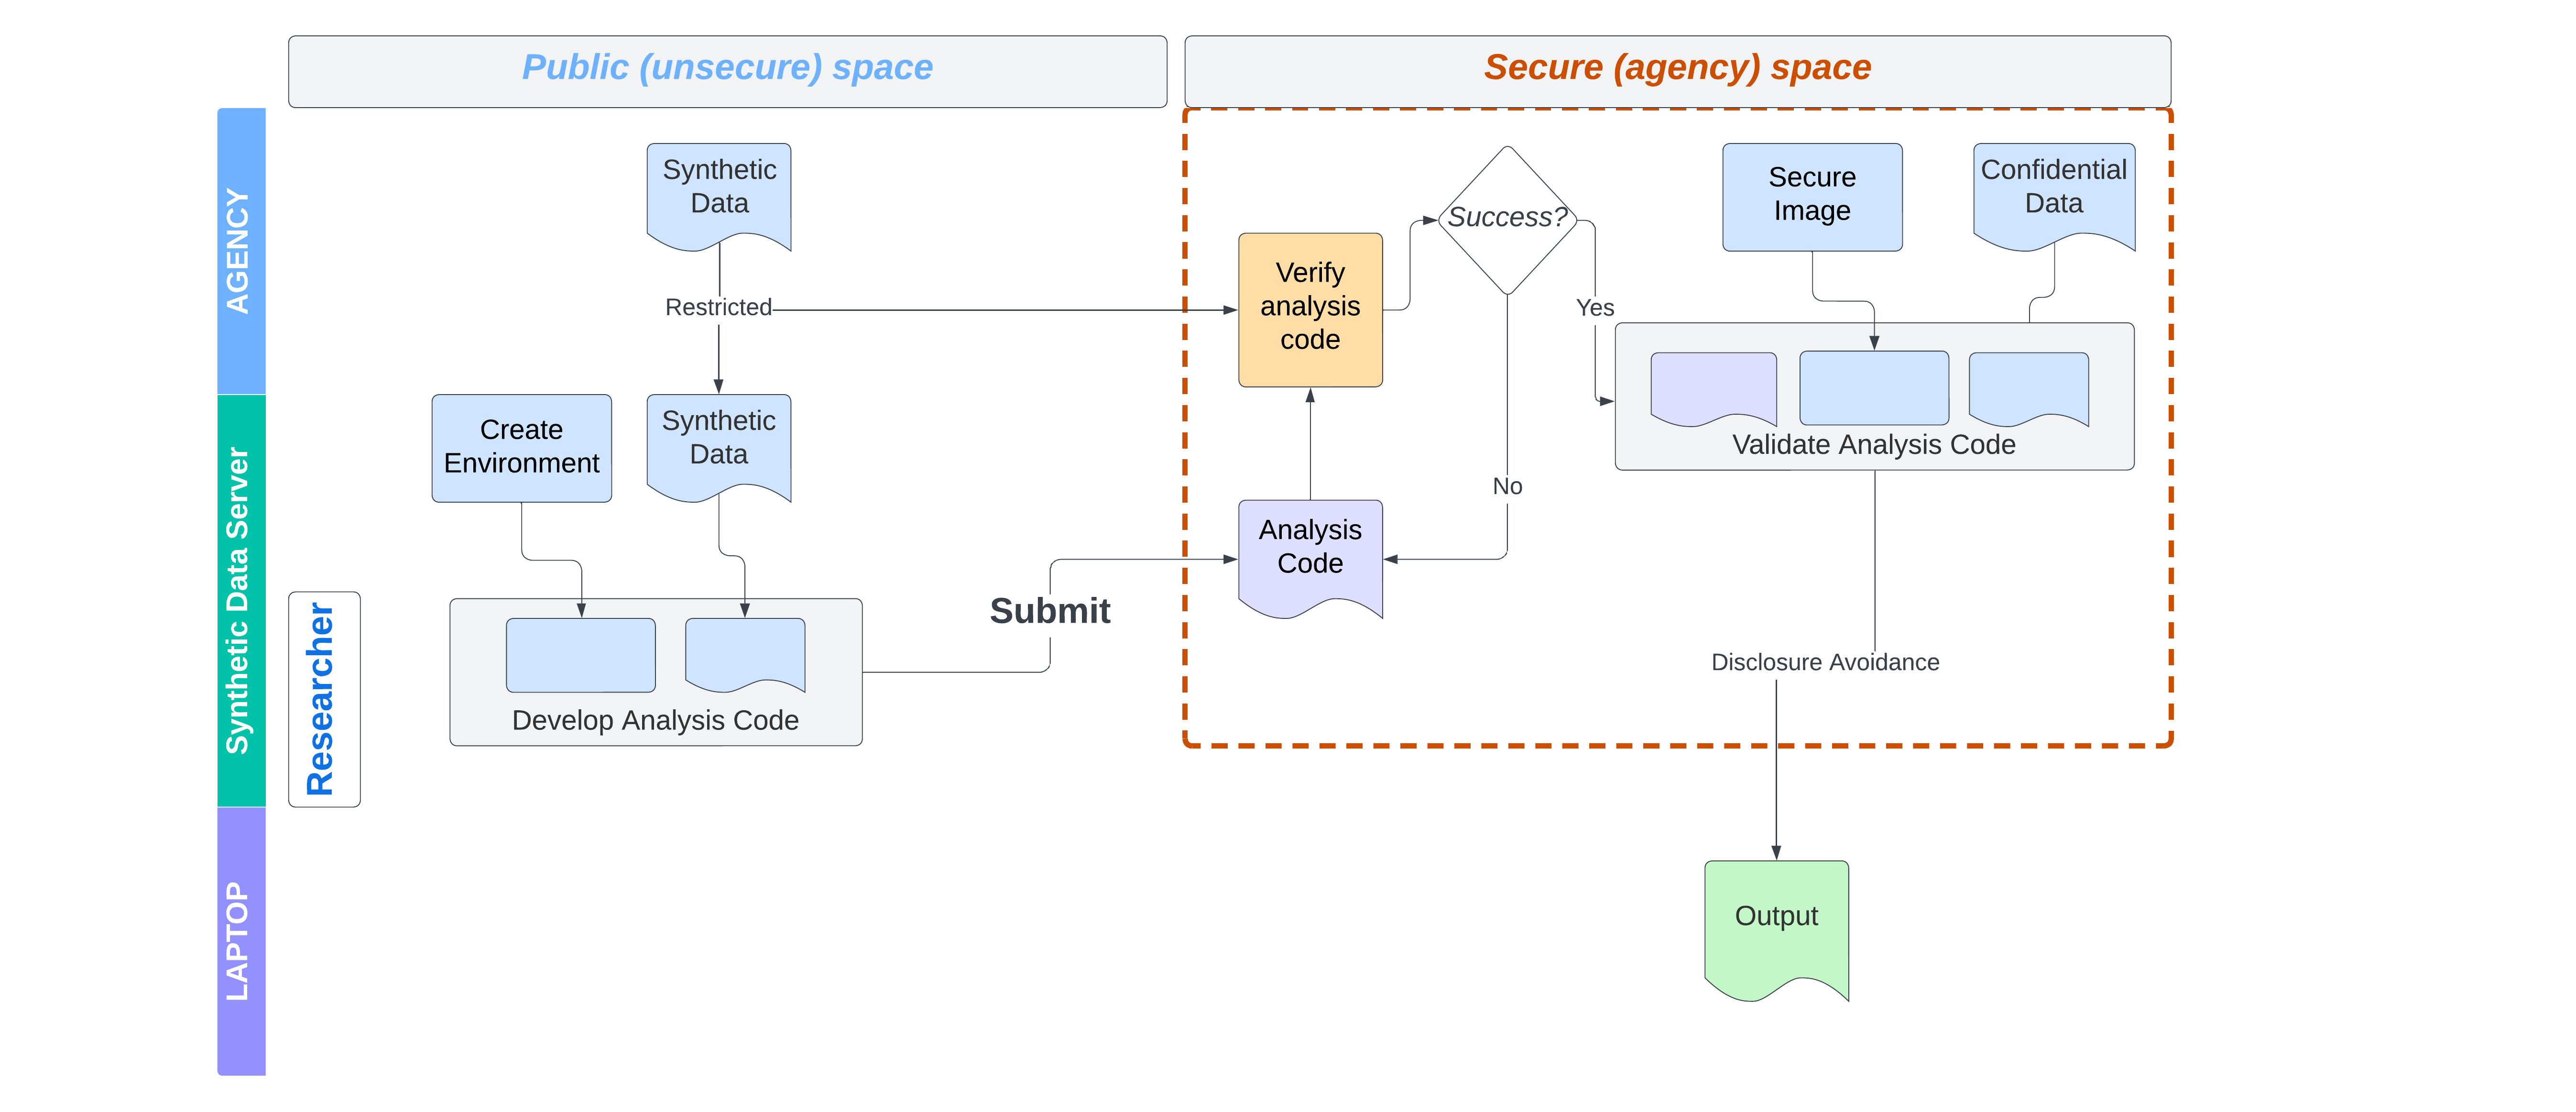
\includegraphics[width=0.45\textwidth]{figs/SSB Flow.png}
\caption{\label{fig:comparision}Old and new Figure 1}
\end{figure}

%\subsection*{To editor}
\textbf{To editor} 

\begin{referee}
As you can see from the three reports attached,
the reviewers are generally positive about the topic, but have a number of non-trivial concerns and
suggestions on the substance (especially from Reviewer 1) and on the paper organization and
presentation. Reading it myself I can see why Reviewers 2 and 3 find it difficult to see quickly what the
article is about. I surmise the concept of "container" is not a commonly understood one, and even
after I read its description in Section 5, it is not immediately intuitive why it can protect data privacy at
scale. Of course that reflects my ignorance, and your article is to educate people like me. Although I
am of sample size 1, I'm quite confident that over 50\% of statisticians are as clueless as I am on this
topic. :-)
For people like me, the article would be much more enticing if it starts with defining the container,
and explain it intuitively in what ways it helps to protect data privacy, and can do so at scale. Then
you can discuss why other methods are inferior and in what way. 
\end{referee}

\begin{response}
    I have now added a new introduction that lays out the goal of the article, and then added/reformated a section on concepts and prior science, which should hopefully address this point.
\end{response}

\begin{referee}
By the way, the list of desiderata in
Section 6 is great,
but I am a strong believer of the no-free lunch principle. I'd be very happy to be wrong here, but
suspect in many practical situations, one may need to prioritize some. If so, some discussions on how
to prioritize may make readers pay more attention to the list, as those who find the list too
demanding or idealistic might choose to ignore it.

\end{referee}

\begin{response}
    This was actually, somewhat obliquely and apparently not clearly, included in the Conclusion:

    \begin{quote}
        Thus, containers satisfy most of the desiderata outlined earlier, but still rely on high-quality synthetic data, and a privacy-protection mechanism that can scale.
    \end{quote}
    
    
    \noindent I address this (hopefully) better in an greatly expanded conclusion/discussion, where I also address many of Reviewer 1's excellent points.

    \vspace{1em} I have also linked the various code fragments more closely to the text, explaining in more detail what they do, for those not necessarily familiar with the code. I have also corrected a few inaccuracies not noted by the referees when describing the setup of the container in the example.
\end{response}


\textbf{Reviewer 1:}

\begin{referee}
    
The manuscript centers on the use of container technology to improve access to confidential data for research while ensuring data privacy and security.  The manuscript outlines how containers, in combination with synthetic data and controlled environments like Codeocean, provide researchers and data stewards with a compatible setup that facilitates statistical analysis on confidential datasets while preserving privacy.  The manuscript discusses how containers create reproducible, secure environments that can be deployed on public or private infrastructure, enabling researchers to develop and validate code on synthetic data.  Once validated, this code can be securely transferred to confidential environments for final analysis.  The manuscript emphasizes the scalability, reproducibility, and importance of disclosure avoidance procedures enabled by containers, ensuring sensitive information remains protected throughout the research process.  It also acknowledges that, although the use of containers helps mitigate scalability issues, a major bottleneck in scaling this system will still lie in the need for automated output vetting, which remains a key challenge in disclosure avoidance.
\end{referee}

\begin{response}
    Thank you for the succinct summary, which is better than mine! I have expanded the intro, and included a summary which I hope is as inteligible as yours.
\end{response}

\begin{referee}

The manuscript presents a strong case for using containers to improve access to confidential datasets while preserving privacy.  By using containerization, the approach enhances reproducibility through a standardized environment as researchers can conduct analyses within consistent configurations.  This setup enables data stewards to establish clear boundaries, such as specific software versions and dependencies, which helps ensure a controlled and reproducible workflow.  Managing these parameters creates an environment where analyses can be reliably repeated or validated. The approach aligns well with best practices in secure data handling. The requirement for researchers to provide only their code, combined with the container's capacity to be rebuilt within a secure environment, adds efficiency to the process.  An implementation of this idea by an institution committed to providing access to confidential datasets while safeguarding privacy would be valuable.  


\end{referee}

\begin{response}
    Thank you for that. I hope you are also the reviewer for our grant application.
\end{response}

\begin{referee}

Below are some suggestions to further strengthen the manuscript.

A valuable addition to the manuscript would be a subsection (or adding some paragraphs) discussing metrics that institutions might consider when evaluating the feasibility of container-based secure environments for accessing and analyzing confidential datasets.  Some potential metrics could be:
    \begin{itemize}
        \item Hardware and infrastructure costs associated with supporting container technology, especially if large datasets or complex analyses require substantial computational resources. 
        \item Number of validations that can be completed in a given period of time, such as per week. 
        \item IT personnel costs, as institutions will likely need staff skilled in containerization, data security, and privacy protocols to set up and maintain these environments effectively. 
        \item Learning costs for both internal and external users, including the time and resources required to train users unfamiliar with container technology. 
        \item The types of software, programming languages, and analysis tools that potential users currently rely on.  This information, possibly gathered through a user survey, can guide institutions in configuring containers with compatible software and dependencies. However, institutions may face challenges in surveying a representative sample of potential users. 
    \end{itemize}

\end{referee}

\begin{response}
    Thank you for that suggestion. We did actually include the first two of those metrics in our grant application, and \textbf{I have expanded what was previously called a Conclusion} (somewhat presumptively), which is now \textbf{Discussion}, discussing the desiderata (as requested by the Editor) and these metrics. While I don't (here) expound on the survey for required tools, I do mention that institutions should be aware of the tools being used in the community that they serve, for instance by looking at the distribution of software used in replication packages. 
\end{response}

\begin{referee}

    Compliance with relevant laws.

\end{referee}

\begin{response}
    I did not address this issue explicitly, because I assumed that no laws need to be changed in order to implement this mechanism. I did add a footnote, identifying this assumption, when discussing disclosure avoidance.


    \begin{quote}
        Footnote: I call this ``usual'', since I make no assumptions about changes to existing laws on data confidentiality that an agency is subject to. In order to be implementable, all data access, whether directly or via this new mechanism, must still be compliant with the laws that the agency is subject to, though some re-interpretation of what are permissible uses may be a separate channel to speed up access.
        \end{quote}
\end{response}

\begin{referee}

    The code snippets provided in the document are a valuable addition, moving the discussion from theory to application and giving readers actionable steps to set up their containerized environments.  This hands-on approach makes the concept more accessible, especially for those looking to replicate or test the methods described.  To further enhance clarity, it would be beneficial to include more inline comments within the code snippets to explain relevant lines, particularly for readers unfamiliar with Dockerfile syntax and Stata commands. 
\end{referee}

\begin{response}
    This is a good point, though I subject this to the Editor's filter of how long an article should be. I now explicitly link to the Github repository with the complete example, and have added comments there, as a hopefully acceptable compromise.
\end{response}

\begin{referee}


    The distinction between "reproducible run" and "validating researcher-provided code" in Sections 6.3.2 and 6.3.4 could benefit from further clarification, as these terms may seem similar yet serve distinct purposes.  In Section 6.3.2, the term "reproducible run" appears to refer to an initial execution of code on CodeOcean's infrastructure to confirm that the code runs without technical errors though this does not guarantee that all necessary code has been executed, as sections of code may be commented out or non-functional.  In contrast, Section 6.3.4 describes a "validation" step where the replicator, or data custodian, re-runs the container on synthetic data to ensure reproducibility in a non-secure environment if there are any doubts or if initial validation wasn't completed on CodeOcean.  While someone with a computer science background might quickly understand these nuances, broader audiences might find the distinction confusing. For this reason, it would be beneficial for the manuscript to elaborate on these two steps, clarifying their distinct roles in the reproducibility and validation process. 
\end{referee}

\begin{response}
    This is a good point, though I subject this to the Editor's filter of how long an article should be. I now explicitly link to the Github repository with the complete example, and have added comments there, as a hopefully acceptable compromise.
\end{response}

\begin{referee}

    The document could benefit from addressing ongoing developments in the use of validation servers, particularly those leveraging differential privacy to automate output vetting.  Several research organizations are exploring validation servers because they allow institutions to control how users submit queries and specify the types of output that can be released, facilitating integration with differential privacy.  Implementing a similar approach with containers raises interesting possibilities and potential challenges. For example, it could be feasible to set up containers equipped with OpenDP, enabling users to run analyses with differential privacy settings on synthetic data.  This setup could allow users to test analyses within a "reasonable" privacy budget and compare the outputs against those obtained using standard statistical software that does not employ differential privacy. However, with the proposed approach based on container technologies, there are likely to be significant challenges in automating output vetting through differential privacy within a secure environment. The manuscript should address these challenges if they exist.  Additionally, requiring users to conduct their analyses in OpenDP may introduce a steep learning curve. 
\end{referee}

\begin{response}
    TBD
\end{response}

\begin{referee}


    In a similar vein, instead of choosing between validation servers and containers, there could be potential in integrating these technologies.  For instance, validation servers could be \textit{containerized and distributed across institutions}, allowing researchers to submit queries locally.  These queries could then be routed to a centralized secure environment, such as one maintained by the Census Bureau, ensuring controlled and consistent query processing across institutions.
    Including a discussion of these ideas in the document's discussion section would provide valuable insight into how containers and validation servers could work together to advance secure, scalable access to confidential data, and automatic output vetting.
\end{referee}

\begin{response}
    The suggestion is intriguing, but highlights issues of trust and certification between institutions - not insurmountable, but also probably not lightweight (as we have investigated in a separate project \url{https://transparency-certified.github.io/} that has not yet written up the ideas).

    For now, I have simply added universities in the discussion:

    \begin{quote}
        Providing evidence of successful reproducibility (validation) may require the use of third parties, such as aforementioned commercial providers, but also universities or other research institutions. 
    \end{quote}
\end{response}

\begin{referee}

     There are several minor comments that need to be addressed in the manuscript:
    \begin{itemize}
        \item Ensure all typos are corrected (like Howver) and that all acronyms and initialisms are clearly defined upon first use (like SSB, FSRDC). 
        \item There is no reference to Figure 1 in the main text. If possible, the provided diagram in Figure 1 could include information on where containers are used or rebuilt to clarify the workflow. 
        \item On page 11, the purpose of the sentence, "which runs for about 3 minutes on a 2021-vintage Linux workstation," is unclear.  Consider clarifying its relevance to the reader. 
        \item On page 9, the phrase "(need cite)" appears and should be replaced with an appropriate reference. 
         \item In section 6.3.4, the sentence, "Should the data custodian have doubts about the verified run of the capsule," requires further clarification on why the data custodian might have doubts about the capsule's verified run. 
    \end{itemize}

\end{referee}

\begin{response}
    Response begins here.
\end{response}

\textbf{Reviewer 2:}

\begin{referee}
    Solutions to issues in both researcher access to confidential data and reproducibility of
results are important, and this paper addresses these issues in novel ways and demonstrates very
compelling applications at a federal agency. Even reading the paper carefully it was difficult to discern
the main conclusion and contribution from the various discussions though. Renaming the manuscript
to relate to Census data, or the facilitation of research on synthetic data, might help the reader since
the current title implies a new innovation in HIPAA compliant containers. Nonetheless there should be
a discussion about the relationship of this contribution to the costs of requirements to obtain HIPAA
compliant containers vs relying on synthetic datasets. 
\end{referee}

\begin{response}
    I appreciate the viewpoint, as I had been blissfully ignorant of HIPAA  compliant containers - these are simply not present in any of the discussions in the social science data confidentiality setup that I have been involved in. In economics as much as in sociology and political science, most academics do not even know what containers are, and certainly don't interact with HIPAA in almost any circumstance.

    I have reviewed what one can learn about HIPAA compliant containers, the context in which they are deployed, and identify where there is a connection. As the reviewer managed to glean from my previous version, the context here is not in securing containers, but in using unsecured containers - those that do not need to be secured - to improve access. I reference a few situations - not just HIPAA - where containers are used in secured environments. Most of those that I am aware of are deployed within an entire environment that is secure by whatever rule (not HIPAA, but GDPR or US Government security), and so the internal structure is less important. I hope this properly delineates the current approach from others where containers themselves play a more dominant role.
\end{response}

\begin{referee}
    
After I realized the manuscript was not on
technical developments for containers, I got the impression it was a discussion of human interaction
with a pilot design for an experiment at the Census bureau, but the manuscript
does not take this further. In short the manuscript needs rewriting for improved clarity at the outset,
including clearing stating the purpose of the work, what the work was, and the findings.

\end{referee}

\begin{response}
    I hope that the present rewrite clarifies this, with changes throughout the text.
\end{response}

\begin{referee}
    
There is
related work in applications of the "Common Task Framework" (see Donoho 2024 \url{https://doi.org/10.1162/99608f92.b91339ef})
and using a container as a reproducible pipeline for checking against withheld test data by a federal
agency (e.g. NIST) should be compared to the approach presented here. 

\end{referee}

\begin{response}
    I now relate to the Common Task Framework, but delineate from the challenge paradigm that Donoho (2024) and others reference. In Donoho's classification, this is meant (possibly) for exploratory analysis. 
\end{response}

\begin{referee}

The authors also appear to
be presenting new standards for reproducible research code publication (e.g. section 6.1) yet don't
reference the extensive body of literature on this topic. 

\end{referee}

\begin{response}
    This was absolutely not meant as a new standard for research code publication. There are too many standards already (none of which is followed in the social science literature that I am familiar with). This is meant purely as a requirement of the validation. I have clarified that.
\end{response}

\begin{referee}
    
Ideally a link to their census example can be
included in the manuscript, allowing readers to try out the example. 

\end{referee}

\begin{response}
    I have added a link to the Github repository for the example.
\end{response}


\begin{referee}
The ideas in the manuscript will
generate lots of reader interest if they can be presented more clearly.
\end{referee}

\begin{response}
    Thank you for your feedback!
\end{response}


\textbf{Referee 3}

\begin{referee}
    A definition of containers should be included in the abstract. 
\end{referee}

\begin{response}
    TBD
\end{response}


\begin{referee}
  It should also be included
early in the main body of the text. \end{referee}

\begin{response}
   Excellent point, and I have added it there.
\end{response}


\begin{referee}
At the very least, the author should consider including a short
roadmap paragraph at the beginning of the paper so that readers know what to expect. Right now, as
is written, containers do not appear until Section 5, leaving readers wonder what the paper is really
about before reaching that point.
\end{referee}

\begin{response}
    You are absolutely right, and this has been (hopefully) corrected.
\end{response}


\begin{referee}

2.
The Media Summary seems missing.

\end{referee}

\begin{response}
    TBD
\end{response}


\begin{referee}

3.
Section 2 paragraph 1: SSB is not defined nearby, but rather in Section 6.

\end{referee}

\begin{response}
    Apologies for that oversight.
\end{response}


\begin{referee}
4.
Table 1: It is unclear what each column is about until reading relevant text. It would be helpful to
add some information about the confidence interval overlap, such as "the closer it is to 1 the higher
the utility" in the table caption.
\end{referee}

\begin{response}
    Apologies for that oversight.
\end{response}


\begin{referee}
5.
Figure 1: It is not mentioned in text what Figure 1 is for and about.

\end{referee}

\begin{response}
    The figure was aspirational. I have simplified the figure, and juxtaposed it to the proposed workflow, which hopefully provides additional clarity.
\end{response}


\begin{referee}
6.
Page 5 middle paragraph: The second sentence starts with talking about Statistic Canada and
microdata.no but ends with the 2018 paper.

\end{referee}

\begin{response}
    I'm not sure what this comment refers to. All four examples refer to examples of scaling up access to restricted-access data, and are discussed (very briefly) in the next sentence. (``scale up access to
confidential data. To cite a few examples,...'' No change was made.
\end{response}


\begin{referee}

7.
Page 5 last paragraph: The author talks about "social sciences" generically but the reference is
on economics. Some edits should be added.

\end{referee}

\begin{response}
    Thank you for pointing that out. The reference is to economics replication packages, since that provides a measurable statistic. I am not aware of a similar collection effort for sociology or psychology, possibly in part because it is harder to parse each article's reproducible materials at scale. I have added this explanation in a footnote, 

    \begin{quote}
        Footnote: Code run in November 2023, searching for any filename that contained the strings `main' or `master', the most common name used for control code in economics. I am not aware of a similarly comprehensive collection for other social sciences. 
        
        \vspace{0.5em} \noindent Text: This is also my impression from our own efforts at the LDI Replication Lab supporting the AEA Data and Code Availability Policy, though we no longer make a systematic effort to categorize this. 
    \end{quote}
    
    
and expanded the reference to point to the various metastudies documenting reproducibility challenges in sociology, economics, political science, and psychology. 

    \begin{quote}
        Footnote: I define ``interactive computing'' as any sequence of computational codes that must be explicitly --- through edits --- adapted to the environment it is running in, and/or does not have a streamlined workflow that can be triggered from a single file, regardless of workflow technology. Examples of workflow management ``systems'' range from \texttt{make} (1976) \citep{association_for_computing_machinery_acm_2003} to \texttt{Snakemake} \citep{molder_sustainable_2021}, to literate programming tools such as \texttt{Sweave} \citep{Leisch2002SweaveDG} and Quarto \citep{Allaire_Quarto_2024}, to simple concatenated calls to software (canonical \texttt{run.sh}). 
        
        \vspace{0.5em} \noindent Text: Examples abound, and can often be gleaned from the fact that many of the reproducibility meta-studies only succeed in reproducing a small number of studies due to limitations in personnel time.

        \vspace{0.5em} \noindent Footnote: \citet{stockemer_data_2018} note ``lack of organization in code and data presentation was the main reason that we were unable to replicate some results'' in political science articles. \citet{StoddenPNAS2018} notes that only 32\% of packages in Science required only minor or no effort to reproduce, though some of the reasons listed are unavoidable (GPU setup, custom hardware) and not related to workflow issues. For the economics journal studied in \citet{herbert_reproduce_2024}, only 24\% required no change to the code in order to be able to run, even when the ultimate results was full reproducibility.
    \end{quote}


\end{response}


\begin{referee}
8.
Section 6.2: The first sentence seems incomplete.

\end{referee}

\begin{response}
I'm not sure I follow, though I think the sentence is maybe too long. The sentence in the submitted version, this sentence read 
    \begin{quote}
6.2. \textbf{Validating reproducibility}. In its base configuration, Codeocean signals to researchers the
successful completion of a run of the controller script ‘run‘ in the right pane of the user interface,
indicating to the custodian of the confidential data that the code is verified to execute on the
synthetic data.
\end{quote}

I have rewritten this to be grammatically somewhat less complex, but also maybe clearer in what I wanted to convey.

\begin{quote}
    The Codeocean interface signals to researchers the successful completion  of the controller script (called \texttt{run}) in the right pane of the user interface. To the custodian of the confidential data, this indicates that the code is verified to execute without error on the synthetic data. The results produced by this specific run of the controller script, and not any previous interactive run, are the results provided in the ``results'' pane. This is important for scalability and efficiency, as it reduces the need for extensive debugging, on the researcher side, and allows for rapid assessment of basic reproducibility by the data custodian.
\end{quote}

\end{response}


\begin{referee}

9.
Any comments/references/examples with Python?

\end{referee}

\begin{response}
    The example is provided as Stata, because most of the users in economics (the original addressees) are Stata users. However, I now point out that this is purely for illustrative purposes. If desired by the reviewer and editor, an equivalent R example could be constructed as a supplement to the existing Stata-based Github example. A python example would not be useful for social scientists, given the low user base there.
\end{response}